% !TeX spellcheck = da_DK
\subsubsection{Forstærker}
En forstærker kan benyttes til at ændre inputtet til et ønsket output. Dette kan gøres ved at skalere, ændre fortegn, addere og subtrahere. Der findes fire forskellige forstærkningskredsløb til at klare de nævtne opgaver: \cite{Nilsson2011}
\begin{itemize}
\item Inverterende forstærknings kredsløb benyttes til at invertere signalet, samtidig med det skaleres. Inverteringen af signalet betyder at der ændres fortegn på signalet. \cite{Nilsson2011} 
\item Summerende forstærknings kredsløb fungerer ligesom det inverterende forstærknings kredsløb, med den undtagelse at input signaler summeres \cite{Nilsson2011}.
\item Ikke-inverterende forstærknings kredsløb benyttes til kun at skalere input signalet \cite{Nilsson2011}.
\item Differens forstærknings kredsløb benyttes til at trække to input signaler fra hinanden, så det bliver muligt at se forskellen \cite{Nilsson2011}. 
\end{itemize} 

For at forstærke det svage signal, som kommer fra accelerometeret, benyttes en operationsforstærker. En operationsforstærker skalerer input spændingen til en ønsket output spænding. Dette gøres for at opnå et bestemt output, hvis den næste komponent skal bruge et specifikt input, eller for at forstærke svage signaler f.eks. fra sensorer eller fysiologiske signaler. Der kan f.eks. bruges en inverterende forstærker, som ses på \figref{invf}, hvor Vs er det målte signal, der ønsket forstærket og Vo er output. Inputtets forstærkning kaldes gain og er en ratio mellem Rf/Rs, som er de to modstande, der kan ses på \figref{invf}. \cite{Nilsson2011}

\begin{figure}[H]
\centering
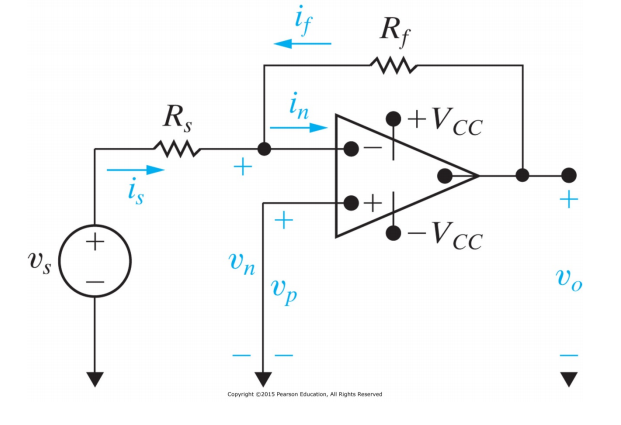
\includegraphics[scale=0.6]{figures/bProblemanalyse/inverterendeforstaerker.png}
\caption{En ideel operationsforstærker, som er inverterende koblet, og som kan forstærke input signalet Vs, til et ønsket output signal Vo. \cite{Nilsson2011}}
\label{invf}
\end{figure}


%INDLEDE MED KORT FORKLARING PÅ HVAD EN FORSTÆRKER EGENTLIG ER OG HVILKE FORSKELLIGE TYPER DER FINDES
%UNDERSTREGE AT VI GODT VED AT DER ER FLERE FORSKELLIGE TYPER AF FORSTÆRKERE..